\documentclass[
  shownotes,
  xcolor={svgnames},
  hyperref={colorlinks,citecolor=DarkBlue,linkcolor=DarkRed,urlcolor=DarkBlue}
  , aspectratio=169]{beamer}
\usepackage{animate}
\usepackage{amsmath}
\usepackage{amsfonts}
\usepackage{amssymb}
\usepackage{pifont}
\usepackage{mathpazo}
%\usepackage{xcolor}
\usepackage{multimedia}
\usepackage{fancybox}
\usepackage[para]{threeparttable}
\usepackage{multirow}
\setcounter{MaxMatrixCols}{30}
\usepackage{subcaption}
\usepackage{graphicx}
\usepackage{lscape}
\usepackage[compatibility=false,font=small]{caption}
\usepackage{booktabs}
\usepackage{ragged2e}
\usepackage{chronosys}
\usepackage{appendixnumberbeamer}
\usepackage{animate}
\setbeamertemplate{caption}[numbered]
\usepackage{color}
%\usepackage{times}
\usepackage{tikz}
\usepackage{comment} %to comment
%% BibTeX settings
\usepackage{natbib}
\bibliographystyle{apalike}
\bibpunct{(}{)}{,}{a}{,}{,}
\setbeamertemplate{bibliography item}{[\theenumiv]}

% Defines columns for bespoke tables
\usepackage{array}
\newcolumntype{L}[1]{>{\raggedright\let\newline\\\arraybackslash\hspace{0pt}}m{#1}}
\newcolumntype{C}[1]{>{\centering\let\newline\\\arraybackslash\hspace{0pt}}m{#1}}
\newcolumntype{R}[1]{>{\raggedleft\let\newline\\\arraybackslash\hspace{0pt}}m{#1}}


\usepackage{xfrac}


\usepackage{multicol}
\setlength{\columnsep}{0.5cm}

% Theme and colors
\usetheme{Boadilla}

% I use steel blue and a custom color palette. This defines it.
\definecolor{andesred}{HTML}{af2433}

% Other options
\providecommand{\U}[1]{\protect\rule{.1in}{.1in}}
\usefonttheme{serif}
\setbeamertemplate{itemize items}[default]
\setbeamertemplate{enumerate items}[square]
\setbeamertemplate{section in toc}[circle]

\makeatletter

\definecolor{mybackground}{HTML}{82CAFA}
\definecolor{myforeground}{HTML}{0000A0}

\setbeamercolor{normal text}{fg=black,bg=white}
\setbeamercolor{alerted text}{fg=red}
\setbeamercolor{example text}{fg=black}

\setbeamercolor{background canvas}{fg=myforeground, bg=white}
\setbeamercolor{background}{fg=myforeground, bg=mybackground}

\setbeamercolor{palette primary}{fg=black, bg=gray!30!white}
\setbeamercolor{palette secondary}{fg=black, bg=gray!20!white}
\setbeamercolor{palette tertiary}{fg=white, bg=andesred}

\setbeamercolor{frametitle}{fg=andesred}
\setbeamercolor{title}{fg=andesred}
\setbeamercolor{block title}{fg=andesred}
\setbeamercolor{itemize item}{fg=andesred}
\setbeamercolor{itemize subitem}{fg=andesred}
\setbeamercolor{itemize subsubitem}{fg=andesred}
\setbeamercolor{enumerate item}{fg=andesred}
\setbeamercolor{item projected}{bg=gray!30!white,fg=andesred}
\setbeamercolor{enumerate subitem}{fg=andesred}
\setbeamercolor{section number projected}{bg=gray!30!white,fg=andesred}
\setbeamercolor{section in toc}{fg=andesred}
\setbeamercolor{caption name}{fg=andesred}
\setbeamercolor{button}{bg=gray!30!white,fg=andesred}


\usepackage{fancyvrb}
\newcommand{\VerbBar}{|}
\newcommand{\VERB}{\Verb[commandchars=\\\{\}]}
\DefineVerbatimEnvironment{Highlighting}{Verbatim}{commandchars=\\\{\}}
% Add ',fontsize=\small' for more characters per line
\usepackage{framed}
\definecolor{shadecolor}{RGB}{248,248,248}
\newenvironment{Shaded}{\begin{snugshade}}{\end{snugshade}}
\newcommand{\AlertTok}[1]{\textcolor[rgb]{0.94,0.16,0.16}{#1}}
\newcommand{\AnnotationTok}[1]{\textcolor[rgb]{0.56,0.35,0.01}{\textbf{\textit{#1}}}}
\newcommand{\AttributeTok}[1]{\textcolor[rgb]{0.77,0.63,0.00}{#1}}
\newcommand{\BaseNTok}[1]{\textcolor[rgb]{0.00,0.00,0.81}{#1}}
\newcommand{\BuiltInTok}[1]{#1}
\newcommand{\CharTok}[1]{\textcolor[rgb]{0.31,0.60,0.02}{#1}}
\newcommand{\CommentTok}[1]{\textcolor[rgb]{0.56,0.35,0.01}{\textit{#1}}}
\newcommand{\CommentVarTok}[1]{\textcolor[rgb]{0.56,0.35,0.01}{\textbf{\textit{#1}}}}
\newcommand{\ConstantTok}[1]{\textcolor[rgb]{0.00,0.00,0.00}{#1}}
\newcommand{\ControlFlowTok}[1]{\textcolor[rgb]{0.13,0.29,0.53}{\textbf{#1}}}
\newcommand{\DataTypeTok}[1]{\textcolor[rgb]{0.13,0.29,0.53}{#1}}
\newcommand{\DecValTok}[1]{\textcolor[rgb]{0.00,0.00,0.81}{#1}}
\newcommand{\DocumentationTok}[1]{\textcolor[rgb]{0.56,0.35,0.01}{\textbf{\textit{#1}}}}
\newcommand{\ErrorTok}[1]{\textcolor[rgb]{0.64,0.00,0.00}{\textbf{#1}}}
\newcommand{\ExtensionTok}[1]{#1}
\newcommand{\FloatTok}[1]{\textcolor[rgb]{0.00,0.00,0.81}{#1}}
\newcommand{\FunctionTok}[1]{\textcolor[rgb]{0.00,0.00,0.00}{#1}}
\newcommand{\ImportTok}[1]{#1}
\newcommand{\InformationTok}[1]{\textcolor[rgb]{0.56,0.35,0.01}{\textbf{\textit{#1}}}}
\newcommand{\KeywordTok}[1]{\textcolor[rgb]{0.13,0.29,0.53}{\textbf{#1}}}
\newcommand{\NormalTok}[1]{#1}
\newcommand{\OperatorTok}[1]{\textcolor[rgb]{0.81,0.36,0.00}{\textbf{#1}}}
\newcommand{\OtherTok}[1]{\textcolor[rgb]{0.56,0.35,0.01}{#1}}
\newcommand{\PreprocessorTok}[1]{\textcolor[rgb]{0.56,0.35,0.01}{\textit{#1}}}
\newcommand{\RegionMarkerTok}[1]{#1}
\newcommand{\SpecialCharTok}[1]{\textcolor[rgb]{0.00,0.00,0.00}{#1}}
\newcommand{\SpecialStringTok}[1]{\textcolor[rgb]{0.31,0.60,0.02}{#1}}
\newcommand{\StringTok}[1]{\textcolor[rgb]{0.31,0.60,0.02}{#1}}
\newcommand{\VariableTok}[1]{\textcolor[rgb]{0.00,0.00,0.00}{#1}}
\newcommand{\VerbatimStringTok}[1]{\textcolor[rgb]{0.31,0.60,0.02}{#1}}
\newcommand{\WarningTok}[1]{\textcolor[rgb]{0.56,0.35,0.01}{\textbf{\textit{#1}}}}
\usepackage{graphicx}
\makeatletter

\usepackage{tikz}
% Tikz settings optimized for causal graphs.
\usetikzlibrary{shapes,decorations,arrows,calc,arrows.meta,fit,positioning}
\tikzset{
    -Latex,auto,node distance =1 cm and 1 cm,semithick,
    state/.style ={ellipse, draw, minimum width = 0.7 cm},
    point/.style = {circle, draw, inner sep=0.04cm,fill,node contents={}},
    bidirected/.style={Latex-Latex,dashed},
    el/.style = {inner sep=2pt, align=left, sloped}
}


\makeatother






%%%%%%%%%%%%%%% BEGINS DOCUMENT %%%%%%%%%%%%%%%%%%

\begin{document}

\title[Lecture 9]{Lecture 9: \\  Bayesian Estimation: Gibbs Sampling}
\subtitle{Big Data and Machine Learning for Applied Economics \\ Econ 4676}
\date{\today}

\author[Sarmiento-Barbieri]{Ignacio Sarmiento-Barbieri}
\institute[Uniandes]{Universidad de los Andes}


\begin{frame}[noframenumbering]
\maketitle
\end{frame}

%%%%%%%%%%%%%%%%%%%%%%%%%%%%%%%%%%%



%----------------------------------------------------------------------%

\begin{frame}
\frametitle{Agenda}

\tableofcontents


\end{frame}
%----------------------------------------------------------------------%
\section{Recap}
\subsection{Bayesian Estimation}

%----------------------------------------------------------------------%
\begin{frame}[fragile]
\frametitle{Bayesian Estimation}

\begin{itemize}


\item {\it Bayes Theorem}

\medskip
\begin{align}
\pi (\beta|X)=\frac{f(X|\beta)p(\beta)}{m(X)}
\end{align}

\medskip
\item with $m(X)$ is the marginal distribution of $X$, i.e.

\medskip
\begin{align}
m(X)=\int f(X|\beta)p(\beta)d\beta
\end{align}
\medskip
\item Bayes' theorem  does not tell us what our beliefs should be, it tells us how they should change after seeing new information.
\end{itemize}

\end{frame}
%----------------------------------------------------------------------%
\begin{frame}[fragile]
\frametitle{Frequentist Approach}

\begin{itemize}
    \item Suppose the model is 
    
    \begin{align}
        y_{i} = \beta x_{i} + u_{i} \\
         u_{i} \sim N(0, \sigma^{2}\ )  \\
        \sigma^{2}\text{ is known}
    \end{align}

    \item Interest is on some form of $h(\beta)$ e.g. $|\beta|$
    \medskip
    \item Frequentists 
    \begin{itemize}
    \medskip
    \item $\hat{\beta}_{MLE}=(X'X)^{-1}X'y$
    \medskip
    \item then use the Delta method (or bootsrap?)
    \end{itemize}
    \medskip
    \item Bayesians
    \medskip
    \begin{itemize}
        \item Using simulation based methods $\rightarrow$ direct sampling algorithm
    \end{itemize}
\end{itemize}


\end{frame}

%----------------------------------------------------------------------% 
\subsection{Direct Sampling}
%----------------------------------------------------------------------%
\begin{frame}[fragile]
\frametitle{Simulation methods}

\begin{itemize}

\item Bayesians specify a prior distribution $\beta \sim N( \beta_{0},  \tau^{2})$
\medskip
\item Use conjugate priors and get the posterior
\medskip
\begin{align}
\beta|\ Y,X\ \sim\ N\ \left(\frac{\frac{1}{\sigma^{2}}\ \sum_{i = 1}^{N}{y_{i}x_{i} + \frac{1}{\tau^{2}}\beta_{0}}}{\frac{1}{\sigma^{2}}\ \sum_{i = 1}^{N}{x_{i}^{2} + \ \frac{1}{\tau^{2}}}},\frac{1}{\frac{1}{\sigma^{2}}\ \sum_{i = 1}^{N}{x_{i}^{2} + \ \frac{1}{\tau^{2}}}}\right)
\end{align}

\item generate $\text{i.i.d.}$ samples from the posterior distribution of $\beta,\ \pi(\beta|Y)$
\item get $h(\beta)$ e.g. $|\beta|$

\end{itemize}
\end{frame}

%----------------------------------------------------------------------%
\begin{frame}[fragile]
\frametitle{Direct Sampling}
\framesubtitle{Example: Linear regression}

\begin{itemize}
\item Goal: posterior mean for $|\beta|$ (quantile $t=50$)
\medskip

\item I generate data $y_{i}$ $x_{i}$ with
\begin{itemize}
\item $ y_{i} = \beta x_{i} + u_{i},\ \text{\ \ u}_{\text{i\ }}\sim\ N\ (0,\ \sigma^{2})$

\item $N = 20$

\item $\beta_{\text{true}} = - 1\ and\ \sigma^{2} = 1$

\item $\beta_{0} = 0\ and\ \tau = 100$
\end{itemize}
\end{itemize}

\begin{figure}[H] \centering
  \centering
  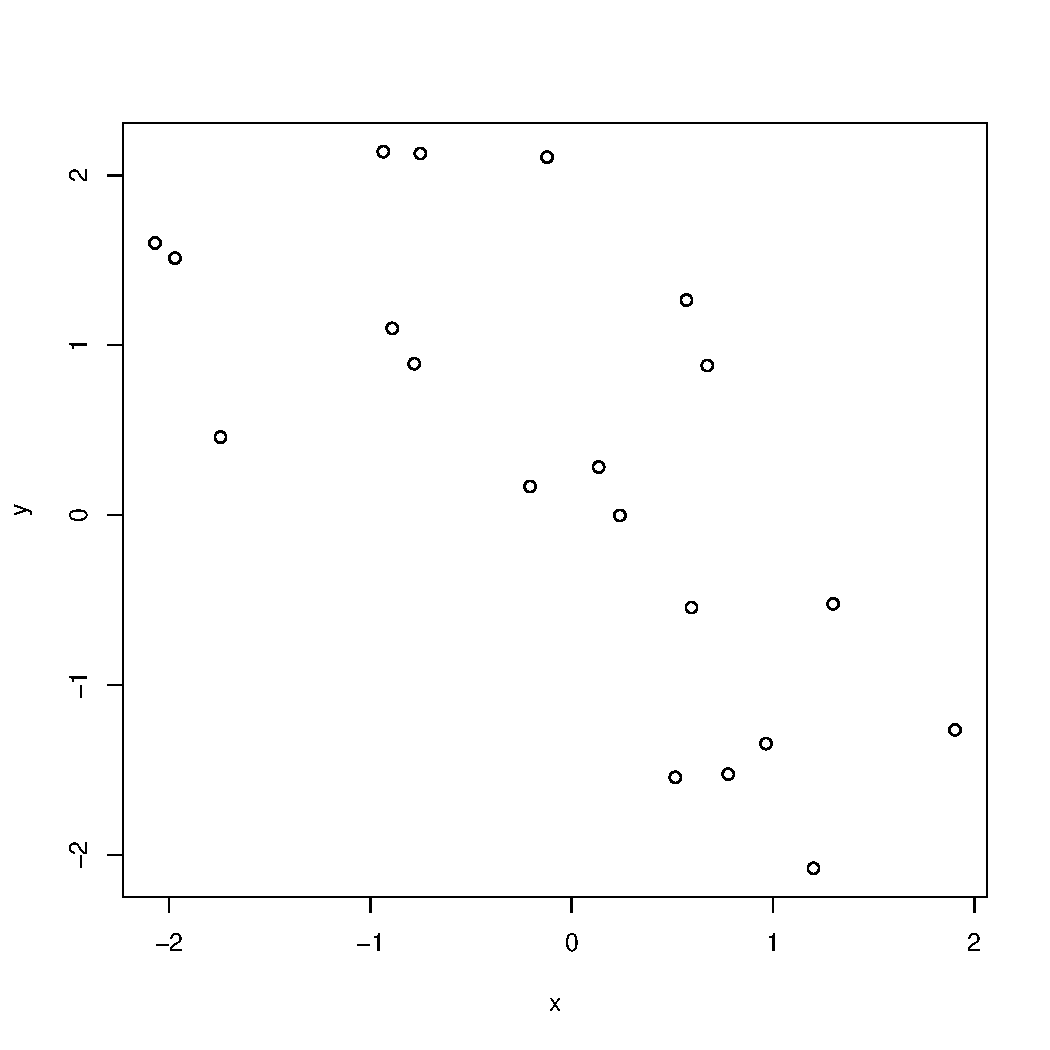
\includegraphics[scale=0.25]{figures/scatter}
  \\
  \tiny 
\end{figure}
\end{frame}
%----------------------------------------------------------------------%
\begin{frame}[fragile]
\frametitle{Direct Sampling}  
\framesubtitle{Example: Linear regression}
\begin{itemize}
\item Step 1: we generate S draws from the $N\left( m,V \right),\ \left\{ \beta^{s} \right\} 1,\ldots,S$

\end{itemize}

\begin{figure}[H] \centering
  \centering
  \caption{Example of draws $\left( \left\{ \beta^{s} \right\}_{1,\ldots,S} \right),\ S = 1,000$}
  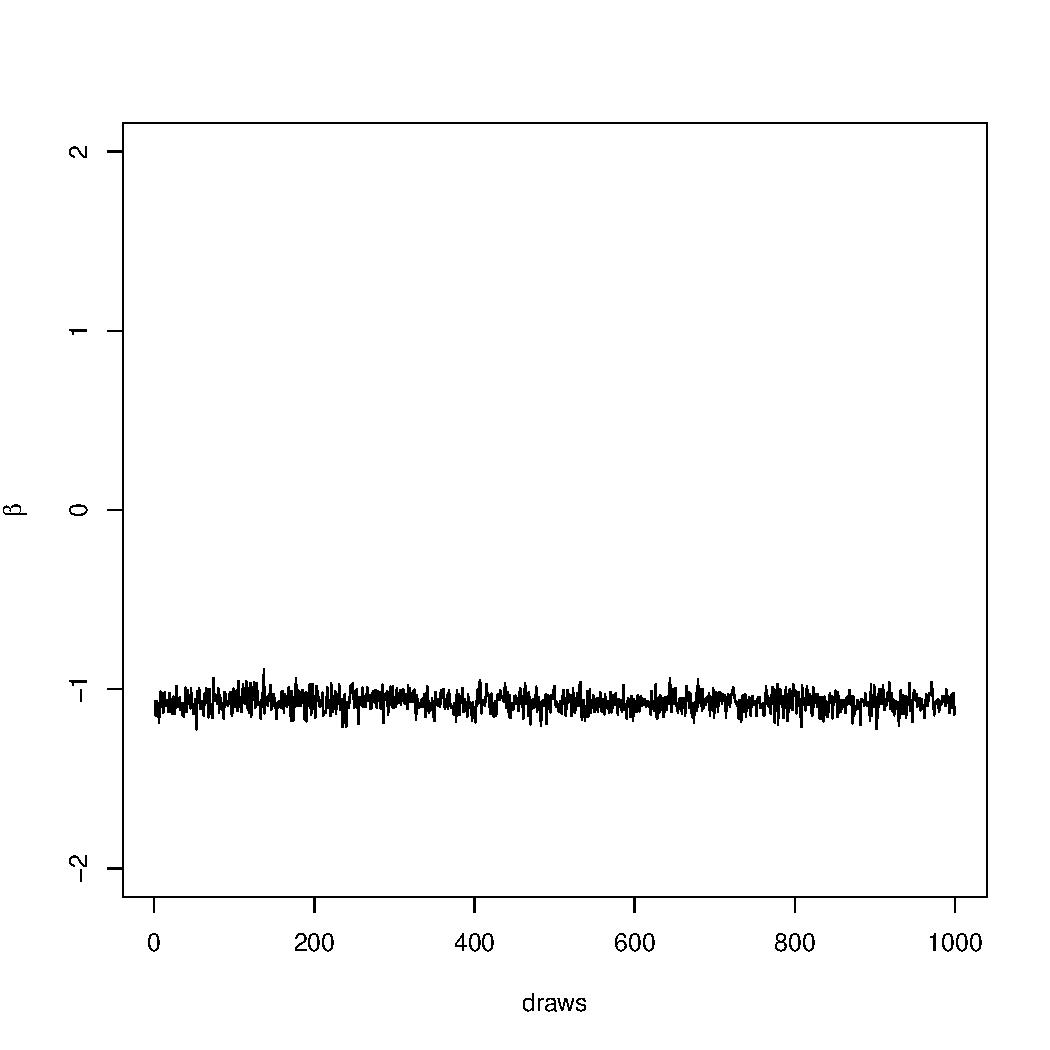
\includegraphics[scale=0.25]{figures/beta}
  \\
  \tiny 
\end{figure}

  
\end{frame}
%----------------------------------------------------------------------%
\begin{frame}[fragile]
\frametitle{Direct Sampling}
\framesubtitle{Example: Linear regression}
\begin{itemize}

\item Step 2: we are interested in posterior moments of $|\beta|$. 
\item Turn draws into $\ \left\{ \left| \beta \right| \right\}_{1,\ldots,S}$
\end{itemize}

\begin{figure}[H] \centering
  \centering
  \caption{Example of draws $\left( \left\{ |\beta^{s}| \right\}_{1,\ldots,S} \right)$}
  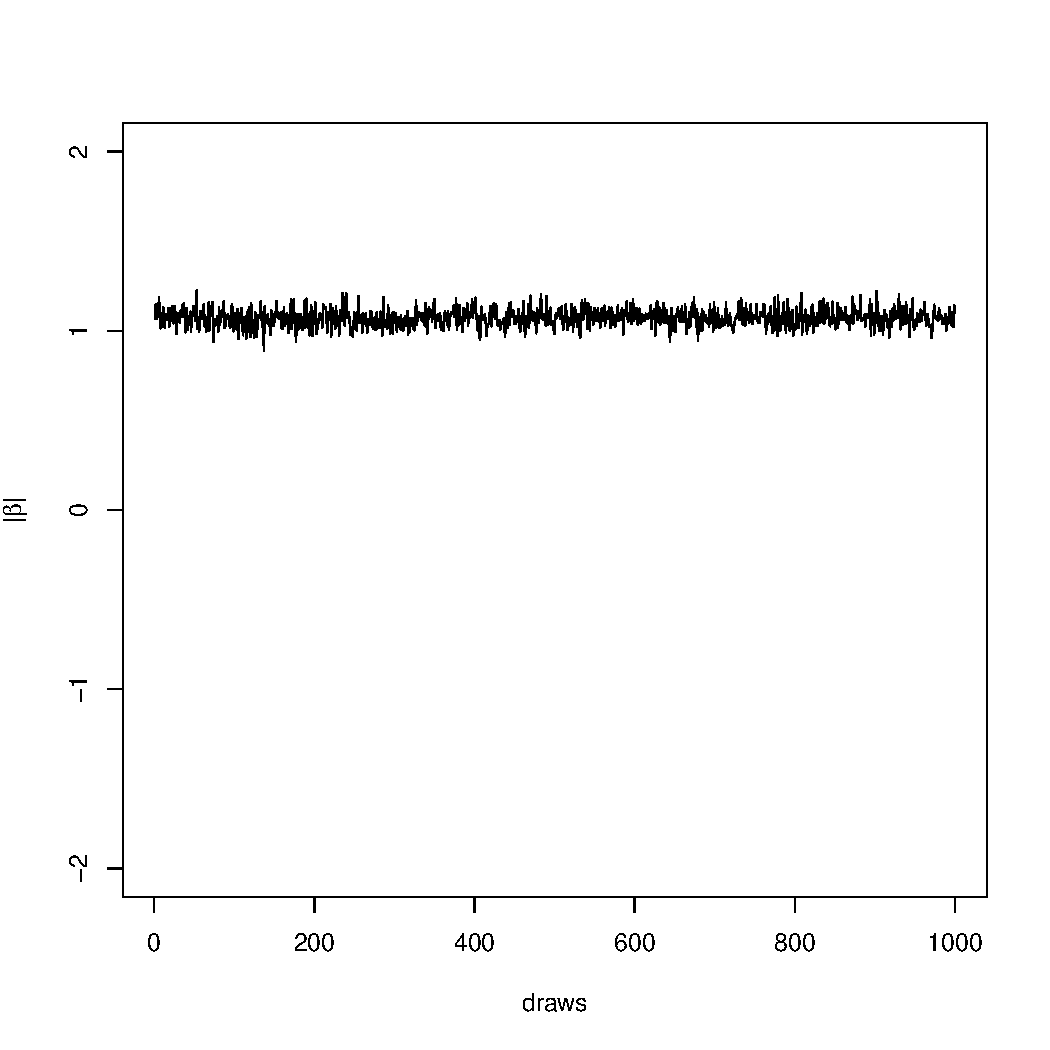
\includegraphics[scale=0.25]{figures/abs}
  \\
  \tiny 
\end{figure}




\end{frame}
%----------------------------------------------------------------------%
\begin{frame}[fragile]
\frametitle{Direct Sampling}  
\framesubtitle{Example: Linear regression}

\begin{itemize}
\item Histogram approximation to $\pi\left( \left| \beta \right|\ |Y \right)$ using $\left\{ \left| \beta^{s} \right| \right\}_{1,\ldots,S}$

  \end{itemize}

\begin{figure}[H] \centering
  \centering
  \caption{Example of draws $\left( \left\{ |\beta^{s}| \right\}_{1,\ldots,S} \right)$}
  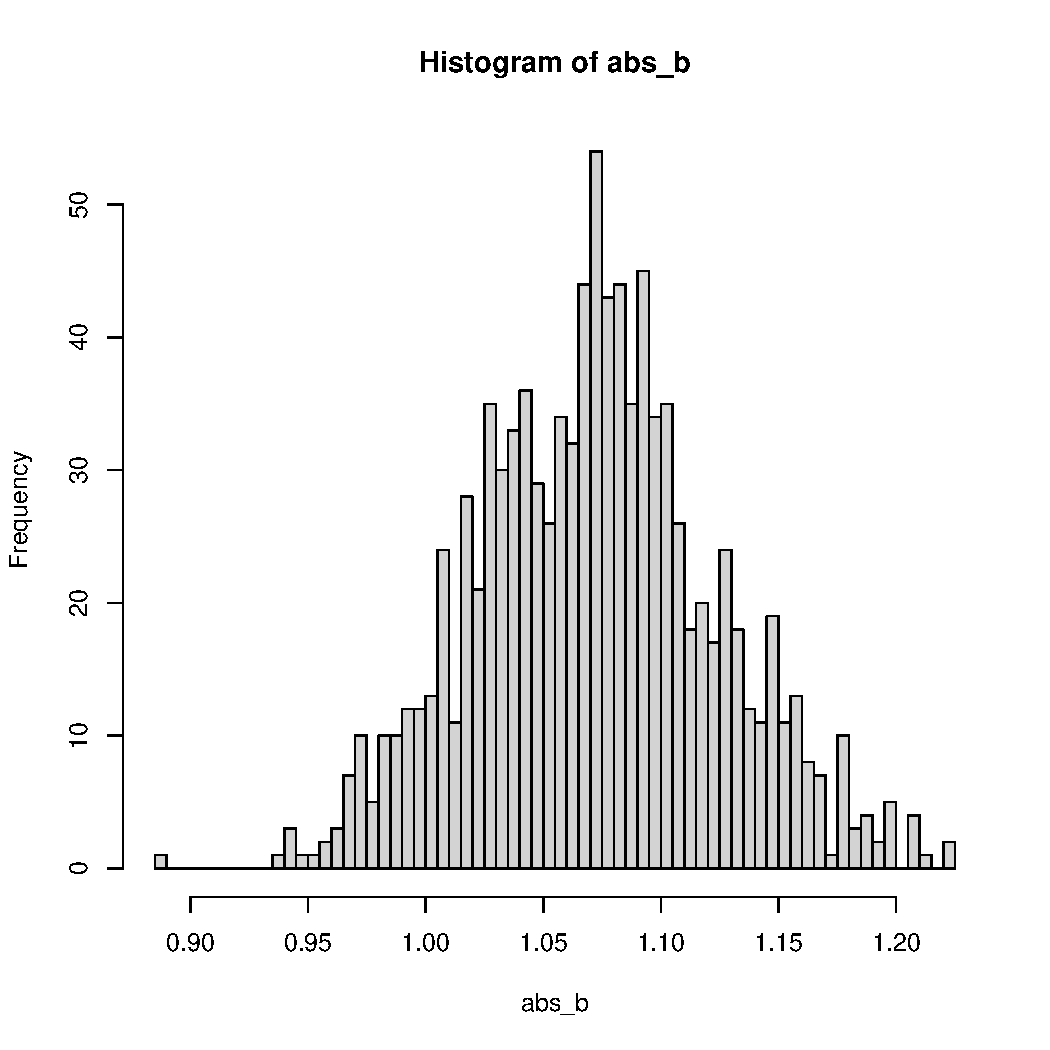
\includegraphics[scale=0.25]{figures/hist}
  \\
  \tiny 
\end{figure}
\end{frame}
%----------------------------------------------------------------------%
\begin{frame}[fragile]
\frametitle{Direct Sampling}  
\framesubtitle{Example: Linear regression}

\begin{itemize}
\item The posterior mean of $\left| \beta \right|$ is approximated by

\begin{align}
E_{Y}^{\beta}\left\lbrack \left| \beta \right| \right\rbrack \approx \frac{1}{S}\ \sum_{s = 1}^{S}{\left| \beta^{s} \right| = 1.0719}
\end{align}

\item Numerical accuracy  use CLT
\end{itemize}


 \end{frame}
 %----------------------------------------------------------------------%
 \section{Gibbs sampling}
%----------------------------------------------------------------------%
\begin{frame}[fragile]
\frametitle{Gibbs Sampling} 


\begin{itemize}

\item Consider now the linear regression model

$$y_{i} = \beta x_{i} + u_{i},\ \ \ \ u_{i}\sim N(0,\ \sigma^{2})$$

\item but assume $\sigma^{2}$ is unknown

\item The prior on $\beta$ is the same as before

$$\beta\ \sim\ N\ (\beta_{0},\ \tau^{2})$$

\item We add now a prior on $\sigma^{2}$ is the Inverse-Gamma

$$\sigma^{2}\ \sim\ IG\ (a,b)$$

\item We want to know the joint posterior distribution

$$\pi (\beta,\ {\sigma}^{2}\ \left| Y,X \right)$$

\item Or we want to know the marginal distribution of $\beta$ and $\sigma^{2}$
\end{itemize}
\end{frame}
%----------------------------------------------------------------------%
\begin{frame}[fragile]
\frametitle{Gibbs Sampling} 



\begin{itemize}

\item We  know the conditional distribution of $\beta$
\medskip
$$\beta|Y,X,\ \sigma^{2}\ \sim\ N\ (m,V)$$
\medskip
\item We can show that
\medskip
$$\sigma^{2}|Y,\beta\,X \sim\ \text{IG}\ \left( a + \frac{N}{2},\ \ b + \frac{1}{2}\ \sum_{i = 1}^{N}\left( y_{i} - x_{i}\beta \right)^{2}\  \right)$$
\medskip

\item That is, IG is conjugate prior for $\sigma^{2}$
\end{itemize}
 \end{frame}
%----------------------------------------------------------------------%
\begin{frame}[fragile]
\frametitle{Gibbs Sampling} 


\begin{itemize}
\item Derivation of the conditional posterior distribution
\medskip
\begin{align}
p ({\sigma}^{2}\left| Y,\ X,\ \beta \right) &\propto p\ \left( Y \middle| X,\ \ \sigma^{2},\ \beta \right)\ p\ (\sigma^{2})\  \\  \nonumber
&\propto \left( \frac{1}{\sqrt{2\ \pi\sigma^{2}}} \right)^{N}\exp\left( - \frac{1}{2}\ \sum_{i = 1}^{N}\frac{\left( y_{i} - x_{i}\beta \right)^{2}}{\sigma^{2}} \right) \times \frac{b^{a}}{\Gamma(a)}\ \left( \sigma^{2} \right)^{- a - 1}\exp\left( - \frac{b}{\sigma^{2}} \right) \\ \nonumber
&\propto \left( \sigma^{2} \right)^{\left( \  - a\  - 1\  - \frac{N}{2} \right)}\exp\left( - \frac{b}{\sigma^{2}} - \frac{1}{2}\ \sum_{i = 1}^{N}\frac{\left( y_{i} - x_{i}\beta \right)^{2}}{\sigma^{2}} \right) \nonumber
\end{align}
(keep terms that are related to $\sigma^{2}$)

\end{itemize}

 \end{frame}
%----------------------------------------------------------------------%
\begin{frame}[fragile]
\frametitle{Gibbs Sampling} 


\begin{itemize}
\item Derivation of the conditional posterior distribution
\medskip
\item We can see that the conditional posterior has the IG density form and we can easily deduce that
\medskip
$$\sigma^{2}|Y,\ \beta\ \sim\ IG\ (\bar{a}\ \bar{b})$$

\medskip
\item  Where

\begin{align}
 \bar{a} &= a + \frac{N}{2} \\ \nonumber
 \bar{b} &= b + \frac{1}{2}\ \sum_{i = 1}^{N}\left( y_{i} - x_{i}\beta \right)^{2} \nonumber
\end{align}

\end{itemize}
 \end{frame}
%----------------------------------------------------------------------%
\begin{frame}[fragile]
\frametitle{Gibbs sampling} 


\begin{itemize}
\item We know conditional posteriors. Can we use these to recover joint distribution?
\medskip
\pause
\item The answer turns out to be yes
\medskip
\item This is very cool. Joint distribution may be nasty and high-dimensional.
\medskip
\item But, Gibbs sampling allows us to break the nasty joint distribution piece by piece

\end{itemize}
 \end{frame}
%----------------------------------------------------------------------%
\begin{frame}[fragile]
\frametitle{Gibbs Sampling} 
\framesubtitle{Example: Linear regression}


\begin{itemize}

\item In the context of linear regression example, the Gibbs algorithm works as below
\medskip
\item Enter the following iteration with $\beta^{0}\ and\ s = 1$
\medskip
\begin{enumerate}
   \item $\left( \sigma^{2} \right)^{s}\ \sim\ p\ (\sigma^{2}|Y,\ \beta^{\left( s - 1 \right)})$
    \medskip

    \item $\beta^{s}\ \sim\ p\ (\beta|Y, \sigma^{(s - 1)} )$
    \medskip
    \item Go to step 1 with $i = i + 1\ $if $i < S$. Otherwise, exit loop
    \end{enumerate}
    \medskip
\item At the end of the algorithm, you get draws $\left\{ \beta^{(s)},\ \left( \sigma^{2} \right)^{(s)} \right\}_{s = 1,\ldots,S}$.

\end{itemize}

 \end{frame}
%----------------------------------------------------------------------%
\begin{frame}[fragile]
\frametitle{Gibbs Sampling} 
\framesubtitle{Example: Linear regression}

\begin{itemize}
\item Under regular conditions,
\medskip
$$ \frac{1}{S - S_{0}}\ \sum_{s = S_{0 + 1}}^{S}{h\left( \beta^{(s)},\ \left( \sigma^{2} \right)^{(s)} \right)}\  \rightarrow_{\text{a.s.}}\ \int_{}^{}{h\left( \beta,\ \sigma^{2} \middle| Y \right)d\beta d\sigma^{2}}$$
\medskip

\item Where the first $S_{0}$ draws are discarded
\medskip
\item CLT also holds so that we can evaluate the quality of the numerical approximation
\end{itemize}
 \end{frame}
%----------------------------------------------------------------------%
\begin{frame}[fragile]
\frametitle{Gibbs Sampling} 
\framesubtitle{Example: Linear regression}

\begin{itemize}
\item Like before, I generate data $y_{i}$ and $x_{i}$ with


$$y_{i} = \beta x_{i} + u_{i},\ \ \ \ u_{i}\ \sim\ N(0,\ \sigma^{2})$$

\footnotesize
with
\item N = 100

\item $\beta_{\text{true}} = \  - 1$ and $\sigma^{2} = 1$

\item Prior for $\beta:\beta_{0} = 0$ and $\tau = 1$

\item Prior for $\sigma^{2}:a = 10,\ b = 20$
\item Start the algorithm with $\beta^{(0)} = 5$
\end{itemize} 


\begin{figure}[H] \centering
  \centering
  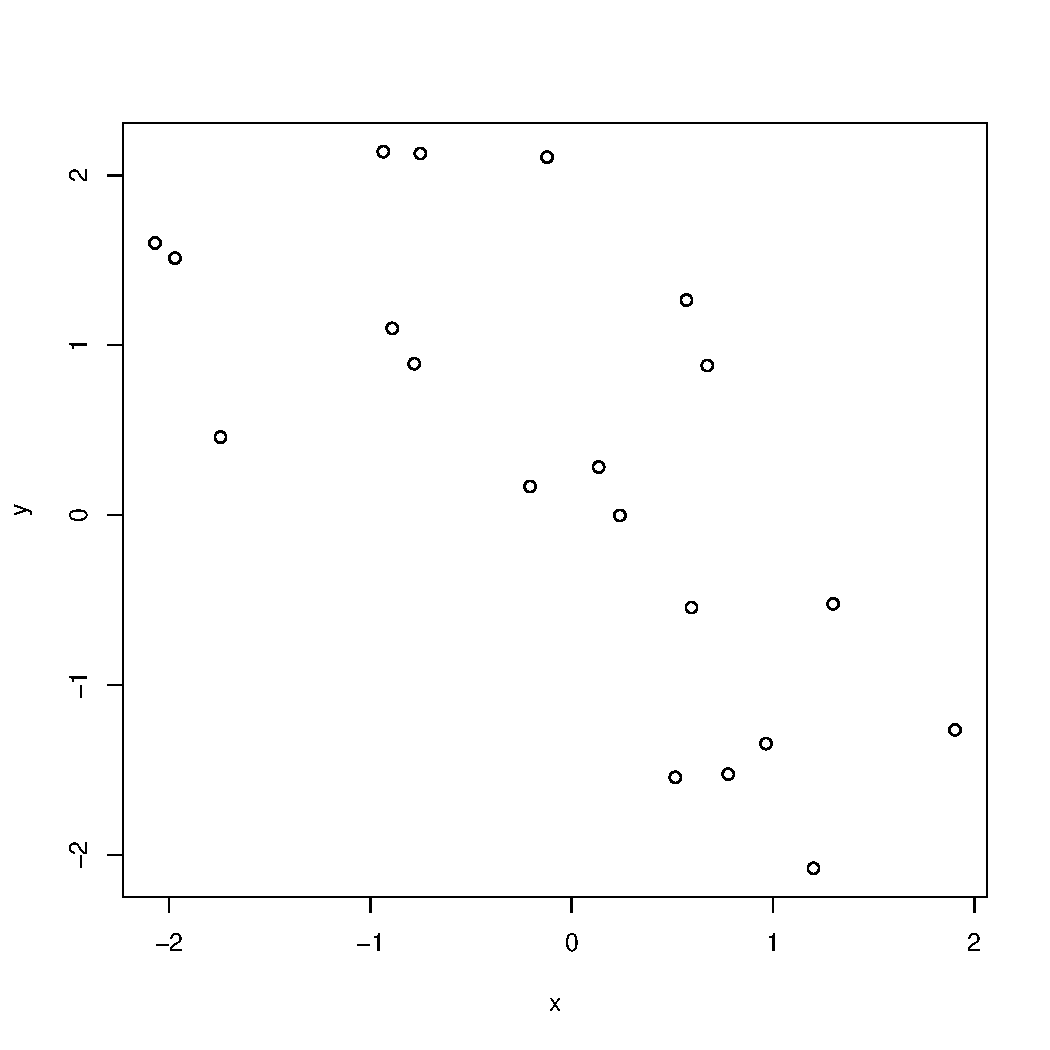
\includegraphics[scale=0.2]{figures/scatter}
  \\
  \tiny 
\end{figure}

   \end{frame}
%----------------------------------------------------------------------%
\begin{frame}[fragile,t]
\frametitle{Gibbs Sampling} 
\framesubtitle{Example: Linear regression}

\begin{itemize}
\item Gibbs sampling: Posterior draws
\end{itemize}
  

\begin{figure}[H] \centering
  \centering
  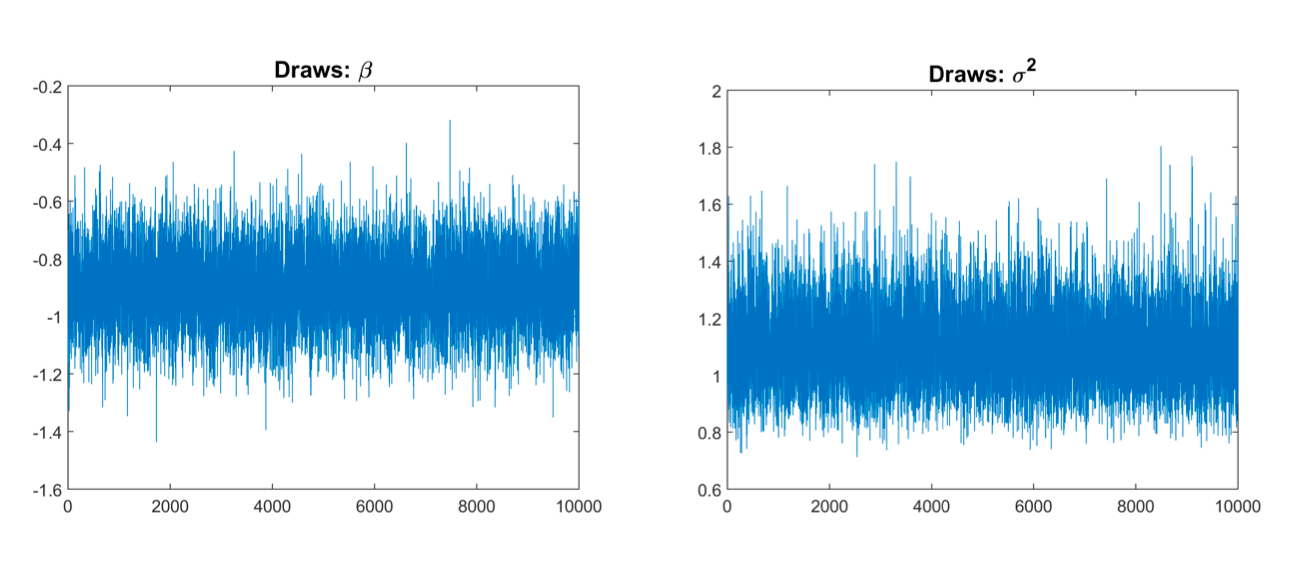
\includegraphics[scale=0.45]{figures/fig1_gibbs}
  \\
  \tiny 
\end{figure}
   \end{frame}
%----------------------------------------------------------------------%
\begin{frame}[fragile]
\frametitle{Gibbs Sampling} 
\framesubtitle{Example: Linear regression}

\begin{itemize}
\item Gibbs sampling: Posterior draws



  
\begin{figure}[H] \centering
  \centering
  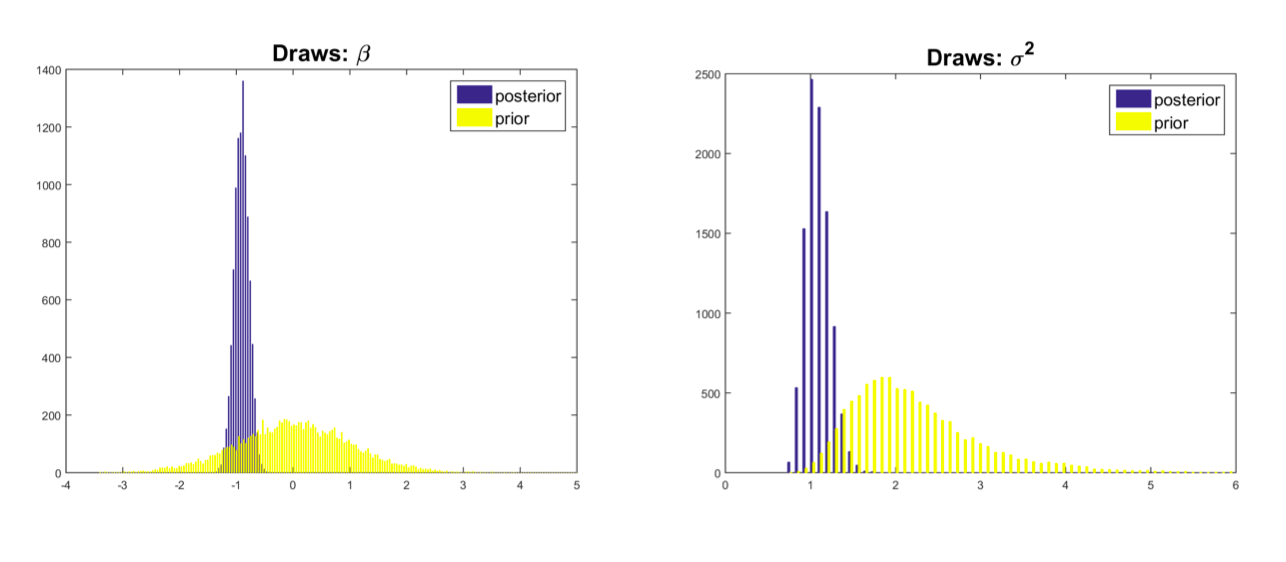
\includegraphics[scale=0.45]{figures/fig2_gibbs}
  \\
  \tiny 
\end{figure}

\footnotesize
\item Once we observe data, we update our belief accordingly.

\item Distribution shrinks. Center of the distribution moved toward where the data generated from:

\begin{align}
\beta_{\text{true}} &= \  - 1 \\
\sigma^{2} &= 1
\end{align}

\end{itemize}
 \end{frame}
%----------------------------------------------------------------------%
\begin{frame}[fragile]
\frametitle{Gibbs Sampling} 
\framesubtitle{Initial value effect}

\begin{itemize}
\item Initial value effect

\item We start the algorithm with some arbitrary number $\beta^{0}$. Theory tells us that this initial value should not matter in the long run.


   
\begin{figure}[H] \centering
  \centering
  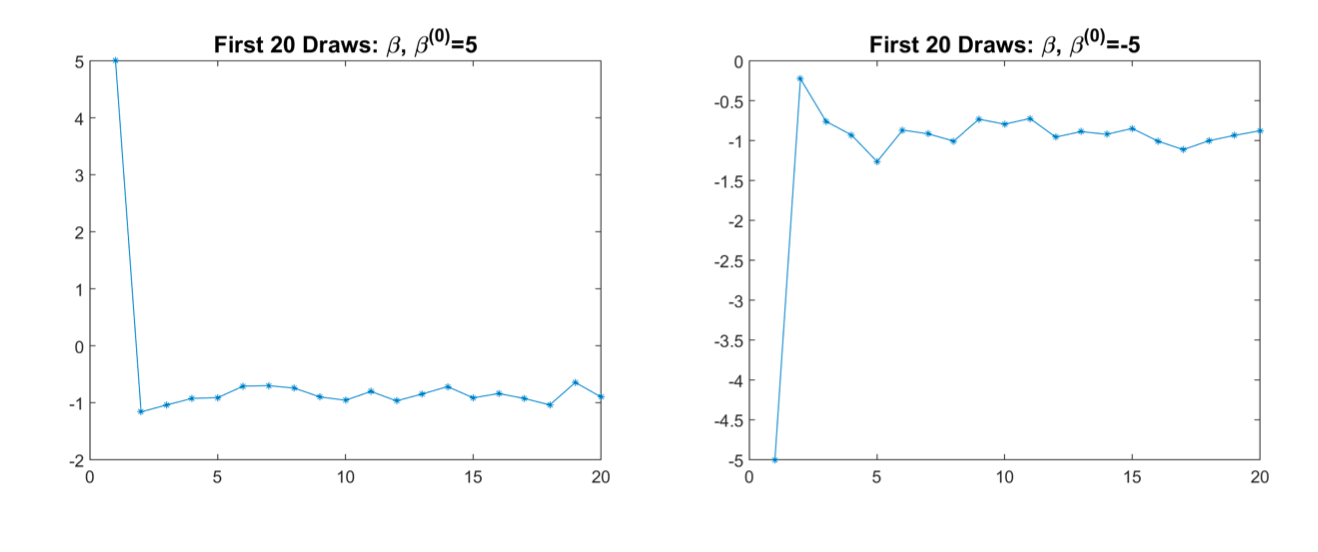
\includegraphics[scale=0.45]{figures/fig3_gibbs}
  \\
  \tiny 
\end{figure}

\item To get rid of the initial value effect, we usually take out first $x$ draws (say, 1,000 draws)
\end{itemize}
 \end{frame}
%----------------------------------------------------------------------%
\begin{frame}[fragile]
\frametitle{Gibbs Sampling} 
\framesubtitle{Checking convergence}

\begin{itemize}
\item Checking convergence
\medskip
\item We start from arbitrary $\beta^{\left( 0 \right)}$
\medskip
\item We can view $\beta^{\left( 0 \right)}$as a draw from the arbitrary distribution (does not have to be the distribution we are interested in).

\item Theory tells us that the sequence from Gibbs algorithm converges to the joint posterior distribution.
\medskip
    \begin{itemize}
        \item After some iteration, $\beta^{\left( i \right)},\ \left( \sigma^{2} \right)^{i}$ is a draw from $\pi\left( \beta,\sigma^{2}|Y \right)^{}$
    \end{itemize}

\item How can we check the convergence? There are many ways.

\end{itemize}

  \end{frame}
%----------------------------------------------------------------------%
\begin{frame}[fragile]
\frametitle{Gibbs Sampling} 
\framesubtitle{Checking convergence: Running Mean Plots}
 
\begin{itemize}
\item Cumulative mean over draws

  \begin{figure}[H] \centering
  \centering
  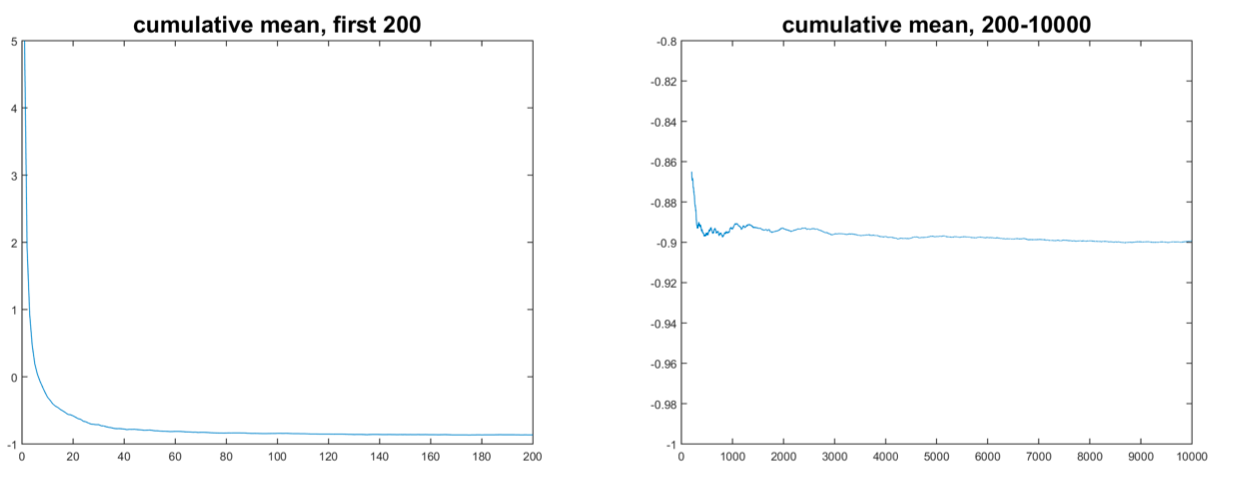
\includegraphics[scale=0.45]{figures/fig4_gibbs}
  \\
  \tiny 
\end{figure}

\item This sequence behaves well in the sense that the Monte Carlo average converges to some number (posterior moment of interest) as the number of
draws increases.
\end{itemize}
 




 \end{frame}
%----------------------------------------------------------------------%
\begin{frame}[fragile]
\frametitle{Gibbs Sampling} 
\framesubtitle{Checking convergence: Geweke's diagnostic check}
 

\begin{itemize}


\item Take out the first $x$ draws

\item  Split draws into two non-overlapping parts (e.g. first 10\% vs last 50\%)

\item Compare Z-score

\begin{figure}[H] \centering
  \centering
  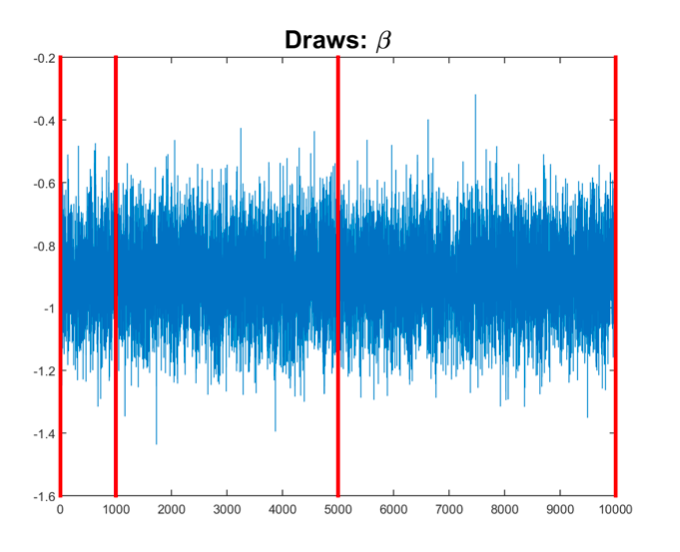
\includegraphics[scale=0.45]{figures/fig5_gibbs}
  \\
  \tiny 
\end{figure}

  
\begin{itemize}
    \footnotesize
\item Standardized mean (Z-score) of the left sample: -6.9363

\item Standardized mean (Z-score) of the right sample: -6.9401

 \item (you can formally test via hypothesis testing).
 \end{itemize}
\end{itemize}
 \end{frame}
%----------------------------------------------------------------------%
\begin{frame}[fragile]
\frametitle{Gibbs Sampling} 
\framesubtitle{Gibbs sampling versus Direct sampling}


\begin{itemize}


    \item A sequence from the Gibbs sampling is serially correlated
    \medskip
    \begin{itemize}
        \item Previous draw affects the current draw.
        \medskip
        \item Gibbs sampler creates a Markov chain. For this reason, it belongs to the class of {\it Markov chain Monte Carlo (MCMC)} procedures.
        \medskip
    \end{itemize}
    \item Recall Direct sampling procedure generates $\text{i.i.d.}$ draws.
\end{itemize}
 
 \end{frame}
%----------------------------------------------------------------------%
\begin{frame}[fragile]
\frametitle{Gibbs Sampling} 
\framesubtitle{Gibbs sampling versus Direct sampling}

\begin{itemize}
\item Both "Direct sampling" and "Gibbs sampling" generate draws that satisfy CLT.

\item For draws from direct sampling:

$$\sqrt{S}\ \left( \frac{1}{S}\ \sum_{i = 1}^{S}h\left( \beta^{i} \right)  - \int{h\left( \beta \right)\pi\left( \beta \middle| Y \right)d\beta} \right)  \rightarrow_{d}\ N\ (0,V_\pi)$$


\item For draws from Gibbs sampling (after discarding first few draws):

$$\sqrt{S}\ \left( \frac{1}{S}\ \sum_{i = 1}^{S}h\left( \beta^{i} \right)  - \int{h\left( \beta \right)\pi\left( \beta \middle| Y \right)d\beta} \right)  \rightarrow_{d}\ N\ (0,V_{G})$$


\item ${V_{\pi} < V}_{G}$

\item To achieve the same level of approximation error, we need more draws $X$ for Gibbs sampler.
\end{itemize}
 \end{frame}
%----------------------------------------------------------------------% 
\section{Review \& Next Steps}
%----------------------------------------------------------------------%
\begin{frame}[fragile]
\frametitle{Review} 
\framesubtitle{General Gibbs sampler}


\begin{itemize}
\item Gibbs sampler works for more than two parameters case. Let be $\theta$ unknown parameter with $\dim{\theta > 1}$



\item Requirements:
    \begin{itemize}
        \item Parameter vector $\theta$ can be partitioned into $\theta =  (\theta_{1},\ \theta_{2},\ \ldots,\ \theta_{m} )$
        \item For each $s$ it is possible to generate draws of $\theta_{s}$ from the conditional distribution, $p\ (\theta_{s}|\theta_{s - 1},\ Y)$ where $\theta_{- s}$ denotes the vector $\theta$ without the partition $\theta_{s}$
    \end{itemize}
    \item Gibbs sampler: For $s = 1,\ \ldots, S:$
    
    \begin{itemize}
        \item Draw $\theta_{1}^{(s + 1)}$ from the density $p\ (\theta_{1}|\theta_{2}^{\left( s \right)},\theta_{3}^{\left( s \right)},\ldots,\ \theta_{m}^{\left( s \right)},\ Y)\ $

        \item Draw $\theta_{2}^{(s + 1)}$ from the density $p\ (\theta_{2}|\theta_{1}^{\left( s+1 \right)},\theta_{3}^{\left( s \right)},\ldots,\ \theta_{m}^{\left( s \right)},\ Y)\ $

        \item $\vdots$

        \item Draw $\theta_{m}^{(s + 1)}$ from the density
        $p\ (\theta_{m}|\theta_{1}^{\left( s+1 \right)},\theta_{2}^{\left( s+1 \right)},\theta_{3}^{\left( s+1 \right)},\ldots,\ \theta_{m - 1}^{\left( s \right)},\ Y)\ $
    \end{itemize}

\end{itemize}




\end{frame}
%----------------------------------------------------------------------%
\begin{frame}
\frametitle{Review \& Next Steps}
  
  \begin{itemize} 
    
  \item  {\bf Next Class:} Empirical Bayes
    \bigskip  
  \item  {\bf Next Week:} PS 2
  
  \end{itemize}


\end{frame}
%----------------------------------------------------------------------%

\section{Further Readings}
%----------------------------------------------------------------------%
\begin{frame}
\frametitle{Further Readings}

\begin{itemize}
  \item Casella, G., \& Berger, R. L. (2002). Statistical inference (Vol. 2, pp. 337-472). Pacific Grove, CA: Duxbury. Chapter 7
  \medskip
  \item Hoff, P. D. (2009). A first course in Bayesian statistical methods (Vol. 580). New York: Springer.
  \medskip
    \item Roberts, G.O. and J.S. Rosenthal (2004): General State Space Markov Chains and MCMC algorithms, Probability Surveys, 1, 20–71.
  \medskip
  \item Geweke, J. (2005): Contemporary Bayesian Econometrics and Statistics, John Wiley \& Sons.
  
\end{itemize}

\end{frame}

%----------------------------------------------------------------------%
%----------------------------------------------------------------------%

\end{document}

%----------------------------------------------------------------------%
%----------------------------------------------------------------------%

